%%%%%%%%%%%%%%%%%%%%%%%%%%%%%%%%%%%%%%%%%%%%%%%%%%%%%%%%%%%%%%%%%%%%%%%%%%%%%%
\section{Run 281: ``ROC buffer overflow'' mode}
%%%%%%%%%%%%%%%%%%%%%%%%%%%%%%%%%%%%%%%%%%%%%%%%%%%%%%%%%%%%%%%%%%%%%%%%%%%%%%
The readout configuration of Run 281 had the event window size of 50 us
and the pulser rate of 60 kHz

\subsection{Hit timing and occupancy}\label{over}
The first distributions to look at are the time distributions of hits in \del{a specific channel}
\add{different channels} and the \del{occupancy} distribution of the total number of hits
in a given channel (occupancy) \del{in}\add{as a} function of the channel number.
The timing distributions of hits \del{in different channels} in channel 0 of the first FPGA
and in channel 2 of the second FPGA are shown in Fig.\ref{fig:1}.
\del{These pictures show the timing distribution of hits .}
The left \del{one}\add{distribution} is, as expected, uniform, however the right one looks
\del{non} \add{less} trivial.

\begin{figure}[H]
  \hspace{-0.5in}
  \begin{tikzpicture}
    \node[anchor=south west,inner sep=0] at (0,0.) {
      % \node[shift={(0 cm,0.cm)},inner sep=0,rotate={90}] at (0,0) {}
      % \makebox[\textwidth][c] {
      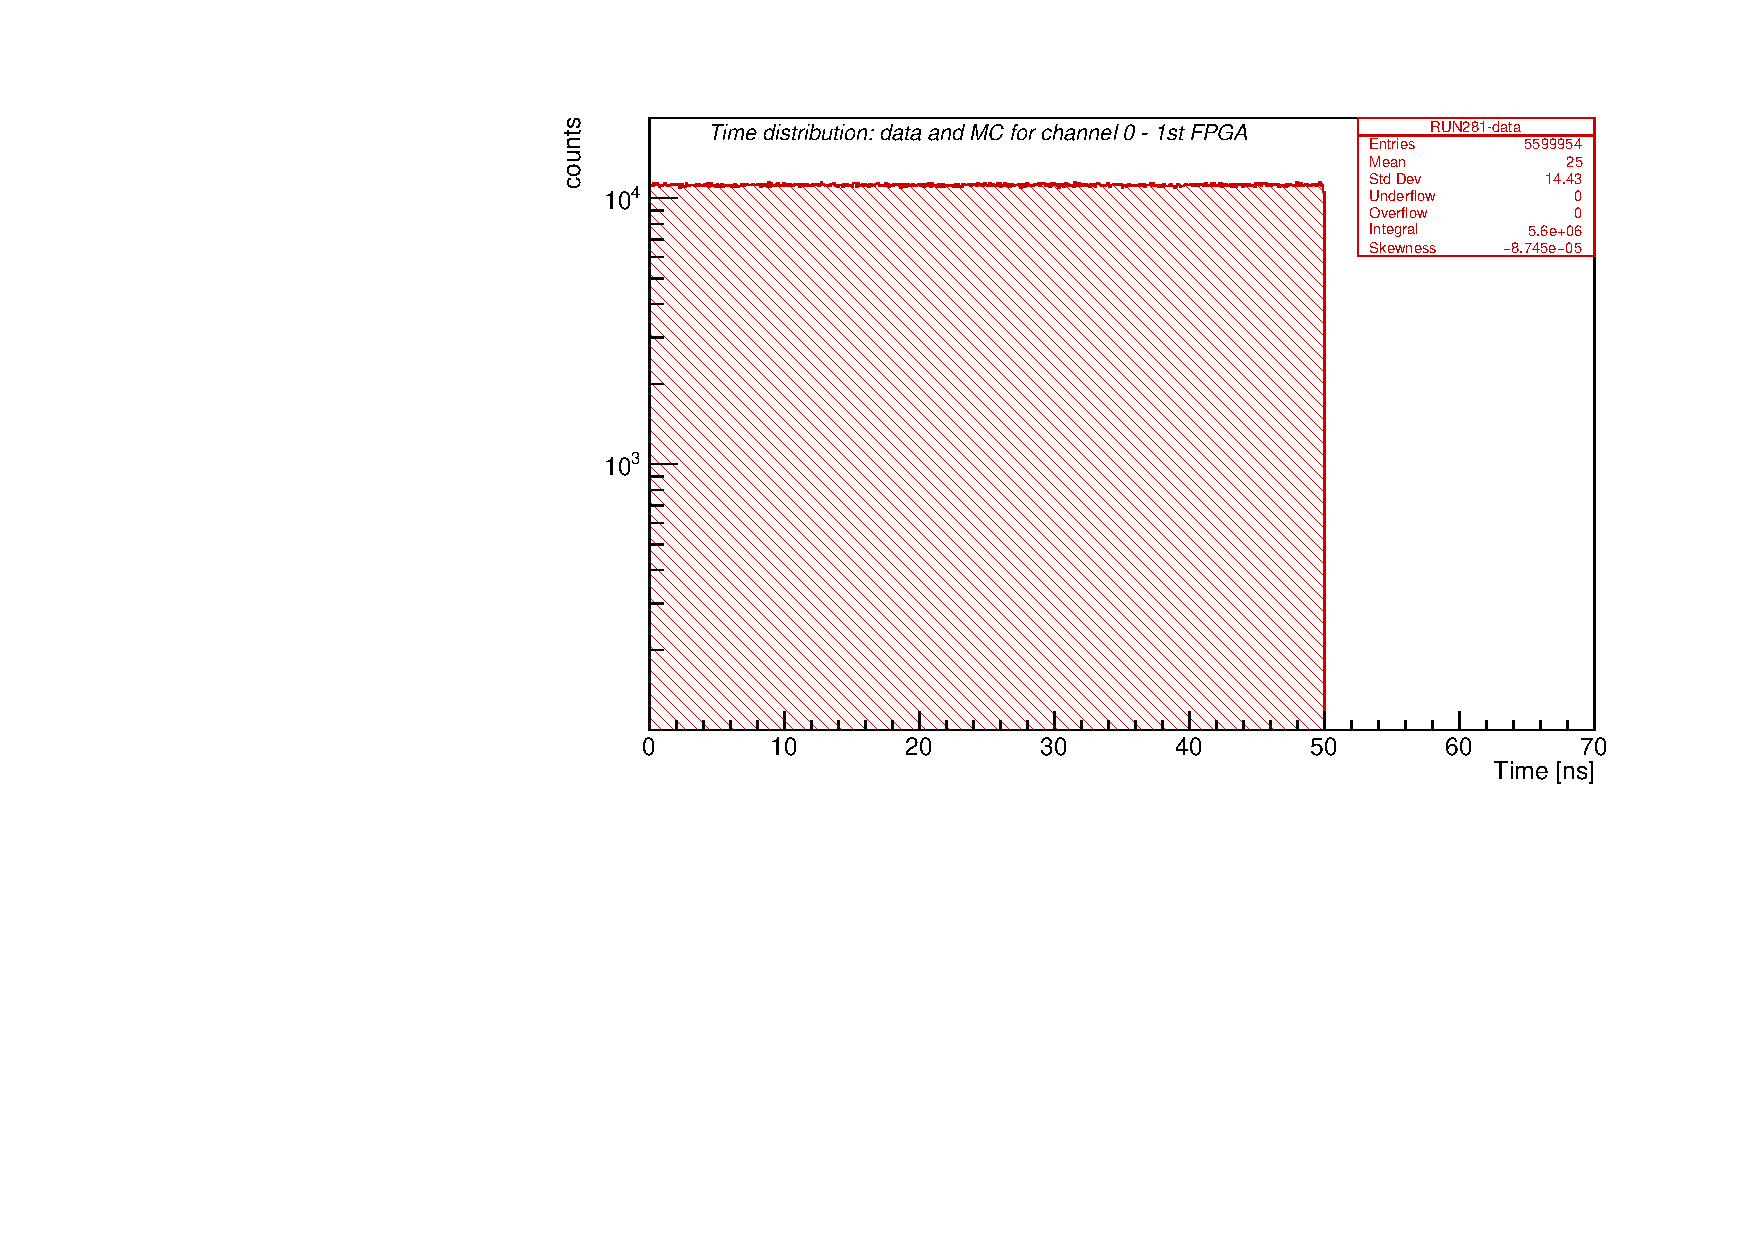
\includegraphics[width=0.5\textwidth]{figures/pdf/figure_00007_timedistr_roc_simulation_ch0_281}
      % }
    };
    \node[anchor=south west,inner sep=0] at (10,0.) {
      % \node[shift={(0 cm,0.cm)},inner sep=0,rotate={90}] at (0,0) {}
      % \makebox[\textwidth][c] {
      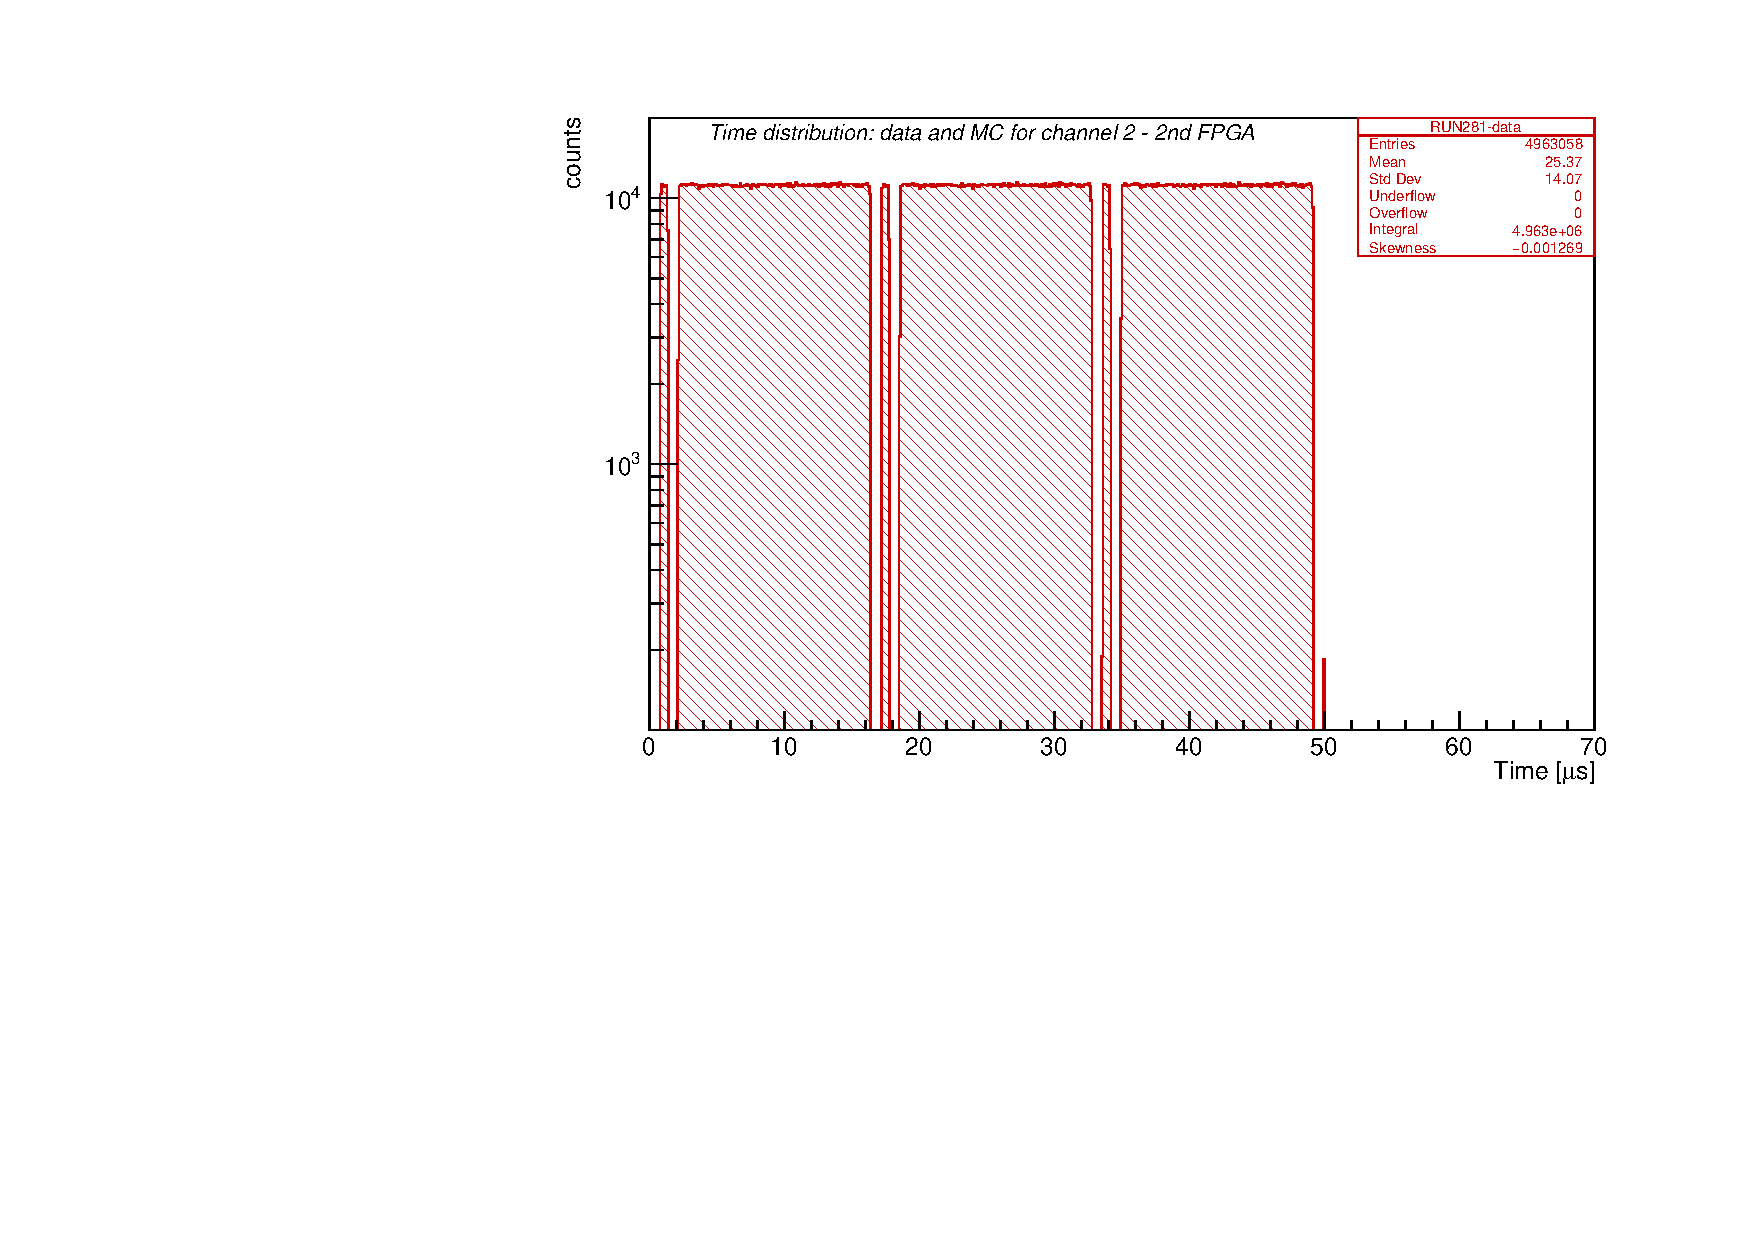
\includegraphics[width=0.5\textwidth]{figures/pdf/figure_00003_timedistr_roc_simulation_ch2_281}
      % }
    };
  \end{tikzpicture}
  \caption{
    \label{fig:1}
    left:
    \del{ channel 0 (first FPGA) time distribution of hits,}
    \add{time distribution of hits in the channel 0, first FPGA}
    right:
    \del{channel 2 (second FPGA) time distribution of hits.}
    \add{time distribution of hits in the channel 2, second FPGA}
    }
\end{figure}

The distributions in Fig.\ref{fig:1} are easier to understand by looking at the occupancy plot in Fig.\ref{fig:2}.left.
\add{The} channel ordering in this plot corresponds to the readout order.
\add{Channels in the beginning of the readout sequence always have all their hits read out,
  however that is not true for the channels in the end of the readout sequence.}
\del{This revealed a non uniform distribution. We compared with the Monte Carlo occupancy.}
\begin{figure}[H]
  \hspace{-0.5in}
  \begin{tikzpicture}
    \node[anchor=south west,inner sep=0] at (0,0.) {
      % \node[shift={(0 cm,0.cm)},inner sep=0,rotate={90}] at (0,0) {}
      % \makebox[\textwidth][c] {
      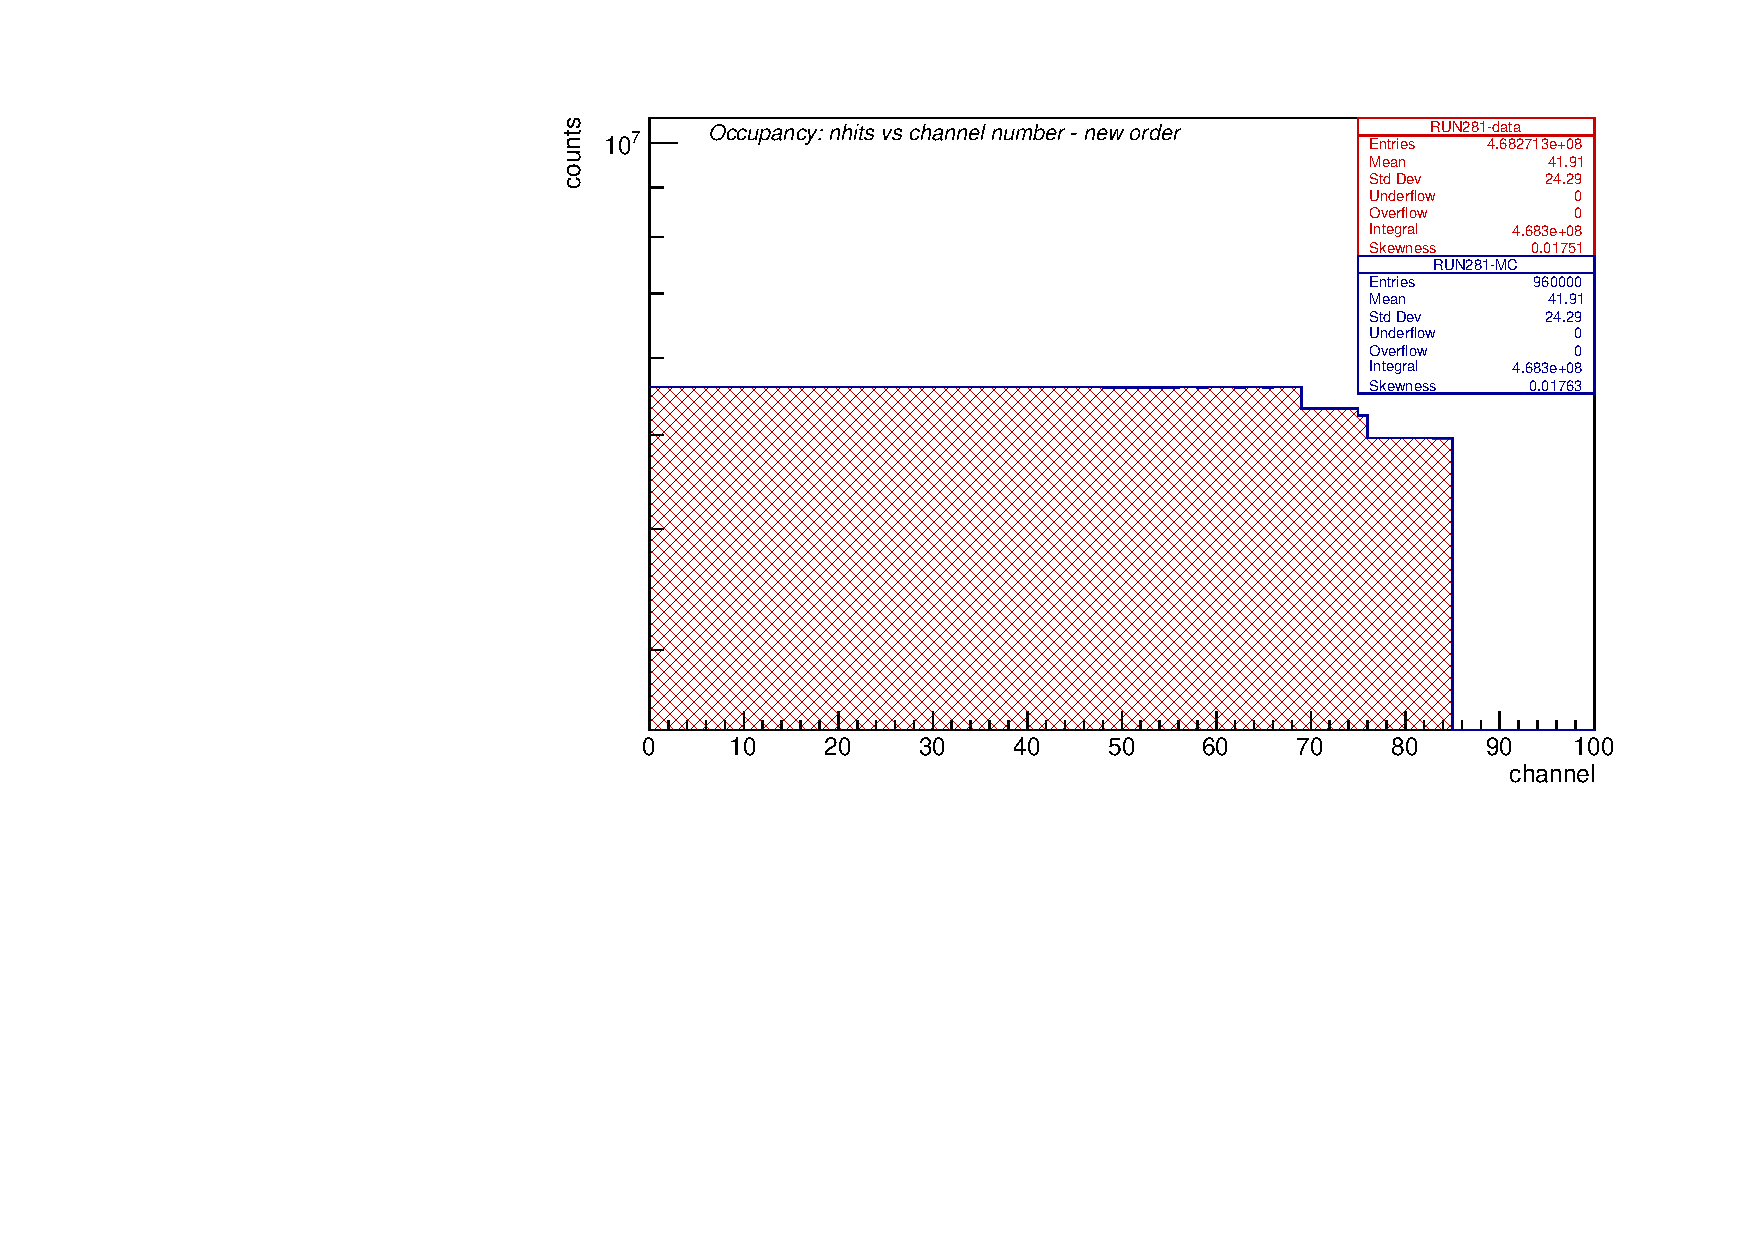
\includegraphics[width=0.5\textwidth]{figures/pdf/figure_00004_nhitsvschannel_roc_simulation_281}
      % }
    };
    \node[anchor=south west,inner sep=0] at (10,0.) {
      % \node[shift={(0 cm,0.cm)},inner sep=0,rotate={90}] at (0,0) {}
      % \makebox[\textwidth][c] {
      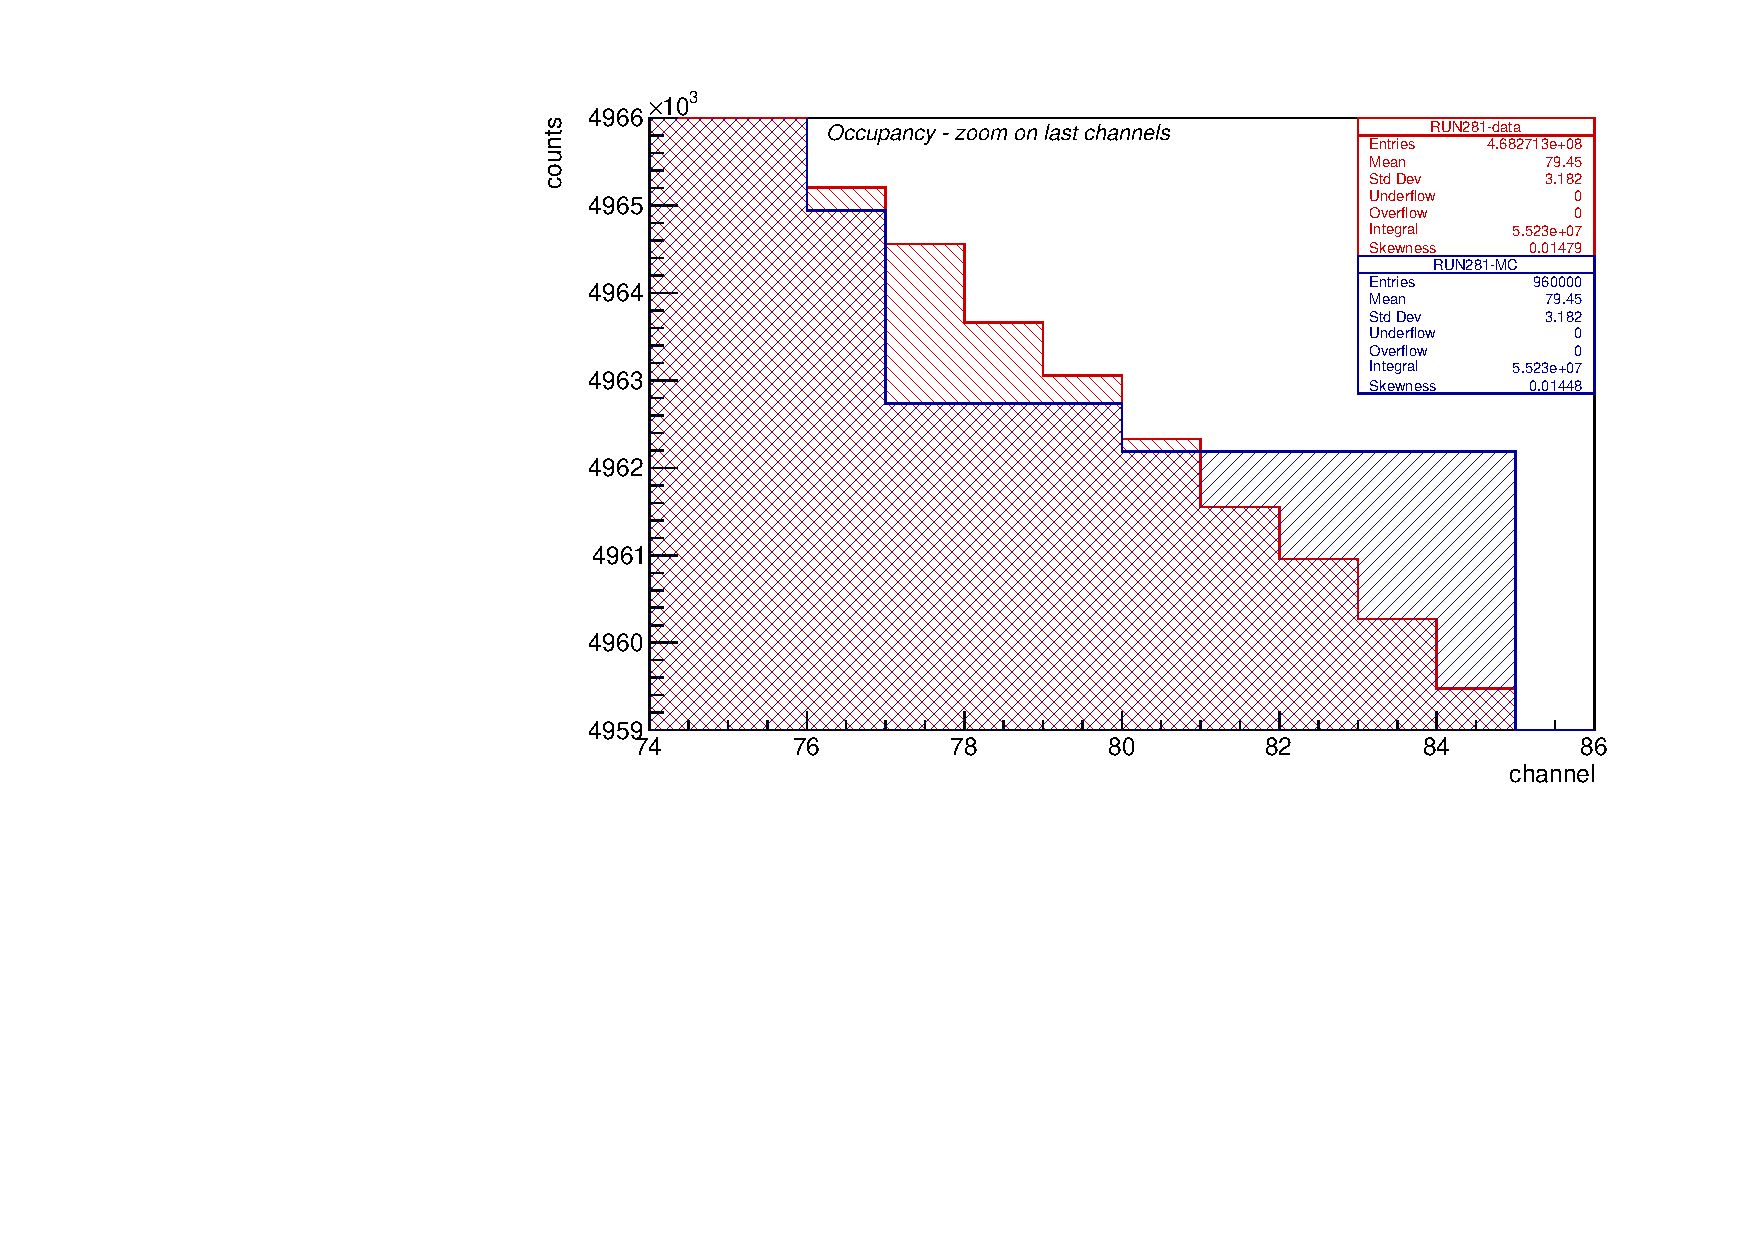
\includegraphics[width=0.5\textwidth]{figures/pdf/figure_00014_nhitsvschannel_roc_simulation_281}
      % }
    };
  \end{tikzpicture}
  \caption{
    \label{fig:2}
    left: number of hits versus \del{channel}\add{the channel number}.
    \del{The ordering of channels adheres to the sequence prescribed by the Monte Carlo simulation,}
    \add{The channels are numbered in the readout order;}
    right: zoom on the last channels in the readout sequence. The \del{two histrograms}\add{data and MC distributions}
    differ from each other \del{of a value <}\add{by $\sim$} 10$^{-3}$.
  }
\end{figure}

\add{Figure \ref{fig:66} shows the distribution of the number of hits in channel 0.
  For the event window of 50 us and the time between the pulses of 16 us, the number of hits could be 3 or 4,
  depending on the timing offset of a given readout window with respect to the generated timing sequence.
  This distribution plays a key role in understanding of the occupancy plot.
}
\del{
  To understand occupancy plot, the number of hits per channel has a key role.
  In Fig.\ref{fig:66} the number of hits (data) in channel 0 is shown. In this configuration
  there could be 3 or 4 hits per channel, as for the other ones.
}
\begin{figure}[H]
\centering
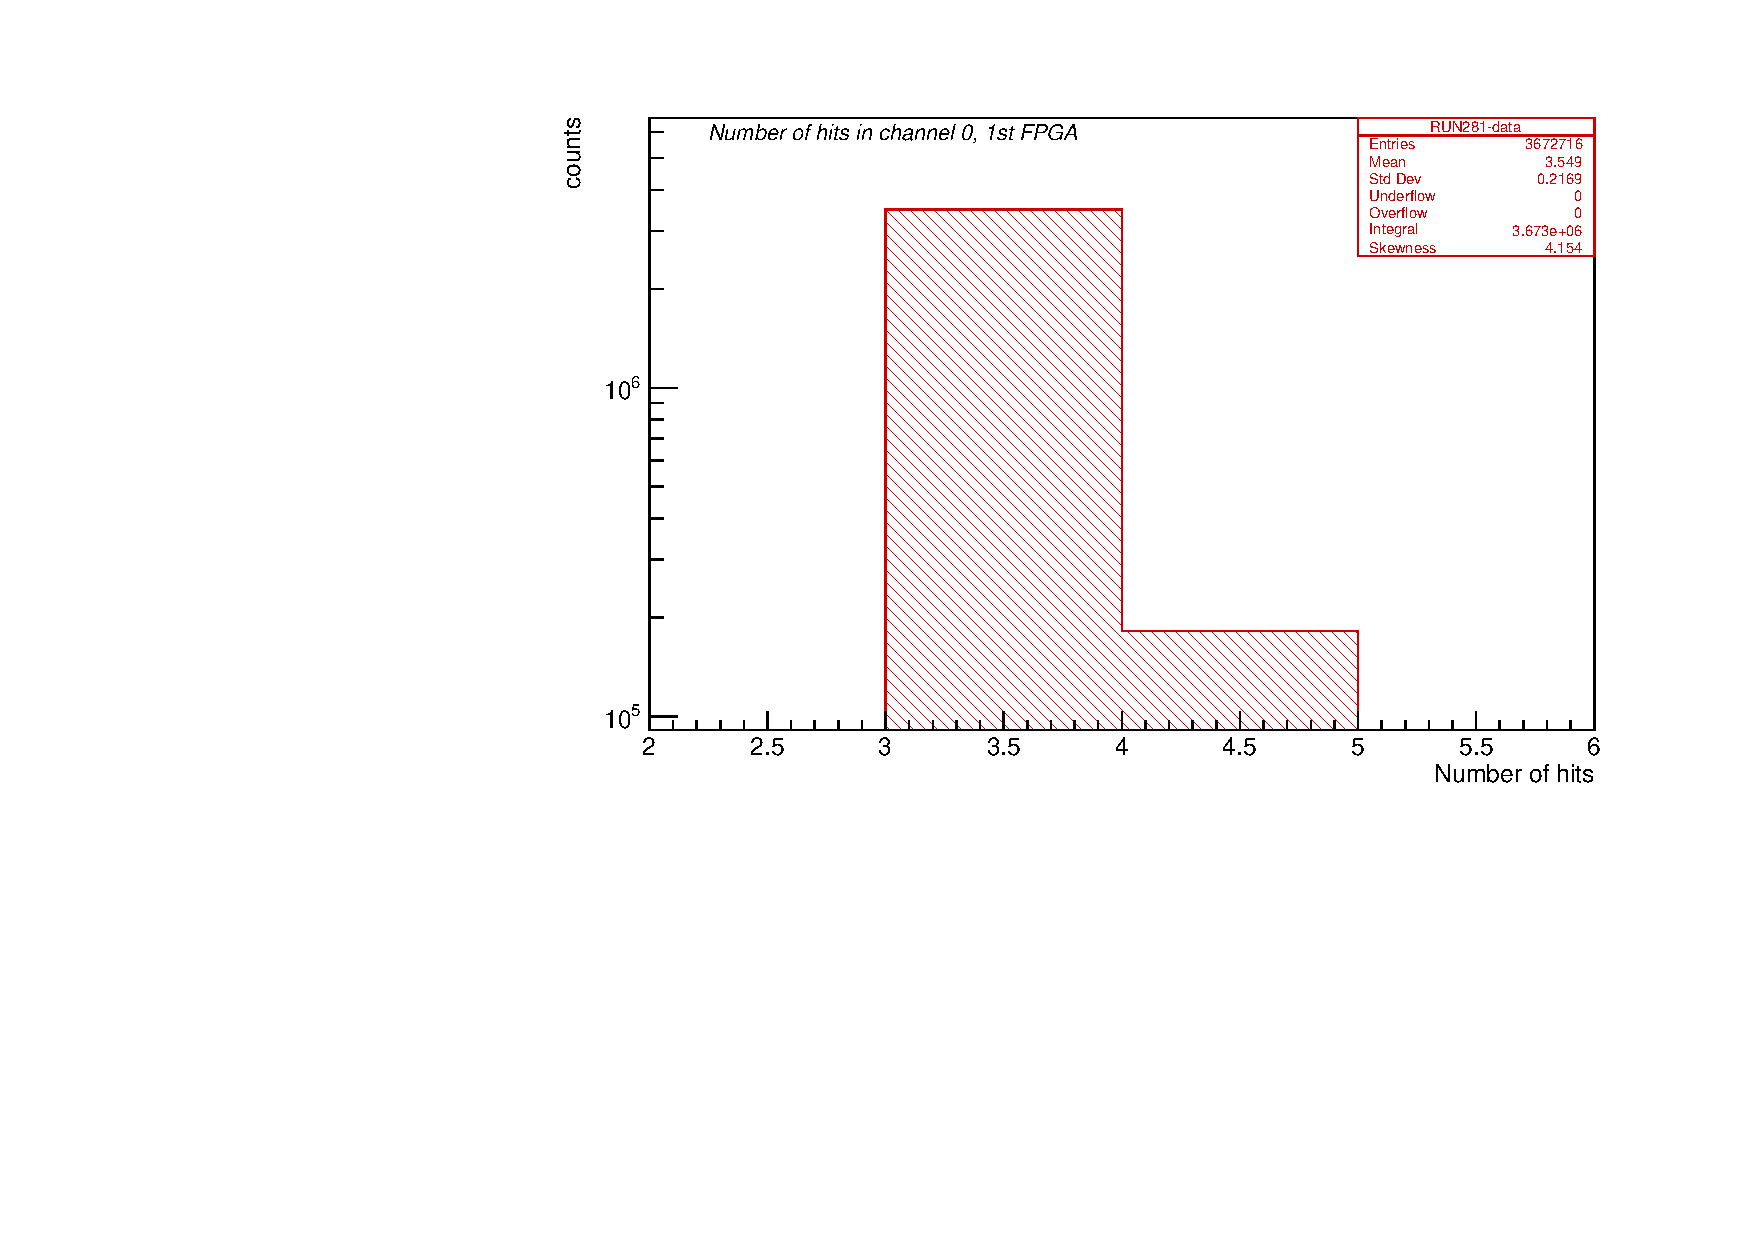
\includegraphics[width =0.8\textwidth]{figures/pdf/figure_00066_nhits_ch00_run281.pdf}
\caption{
  \del{Number of hits per channel. It is shown that in this configuration there could be 3 or 4 hits in channel 0, as in other channels.}
  \add{The distribution of the number of hits in the channel 0 of the first digi FPGA. for run 281}
}
\label{fig:66}
\end{figure}

\add{In the distribution shown in Figure \ref{fig:2}.left,}
\del{In the left picture of Fig.\ref{fig:2},} the first 68 channels are the ones with 4 hits \add{per channel}
in the first FPGA and three \add{hits per channel} in the second FPGA, \del{achieving in total}
\add{resulting in the total of} 255 hits.
The second plateau extending from 68 to 75 \del{is composed by}\add{corresponds to} the channels
with 3 hits \add{per channel} in the first FPGA and 4 hits \add{per channel} in the second one.
\add{
  The ``dent'' in the end of the second plateau is due to the fact that the 48 channels of the first FPGA
  yield 144 hits, so the second FPGA contributes 111 hits. The first 27 channels of the second FPGA contribute
  4 hits per channel each, but as 111 is not an integer of 4, the three hits from channel 28 in the readout sequence
  fill up the total ROC buffer of 255 hits.
}
There is a big step at the end of this plateau, because if we count the number of hits
in the first FPGA we get 144, so in the second FPGA we have 111 hits in total,
due to the fact that the maximum number of hits in total is 255.
111 is not divisible by 4, so the first 27 channels in the second FPGA will have 4 hits
and the last one will have 3 hits.
The last plateau \del{consists of}\add{corresponds to} 3 hits \add{per channel} from the first FPGA
and 3 hits \add{per channel} from the second FPGA.

A zoom on last channels is shown on the right picture of Fig.\ref{fig:2}.
\del{The two histograms differ from each other of a value $<10^{-3}$: this is a}
\add{
  The relative difference between the data and the MC distributions is at a level of $10^{-3}$,
  which is a very
}
good agreement.
\del{
  The differences are due to the fact that each FPGA has its own pulse generator and pulse sequences
  from different generators are offset with respect to each other by a random number and also timing
  of generator pulses are uncorrelated with the beginning of the time window.
}
Coming back to Fig.\ref{fig:1}, \add{the first channels in the readout sequence}\del{some channels are}
always \add{have all their hits} read out \del{and some others no},
\add{while the channels in the end of the readout sequence - do not},
as \del{we explained in the introduction} the ROC hit buffer gets filled up \del{and only}\add{after}
the first 255 hits are read out.
This results in a uniform time distribution for the first channels readout and in a non-uniform
time distribution for the last readout channels, depending on $T_{gen}$ and $T_{EW}$.
The \del{deeps}\add{dips} in channel 2 are defined by the \add{timing offset} \del{differences}
between the two FPGA pulsers. 


%%%%%%%%%%%%%%%%%%%%%%%%%%%%%%%%%%%%%%%%%%%%%%%%%%%%%%%%%%%%%%%%%%%%%%%%%%%%%%
\subsection{Number of hits}
Fig. \ref{fig:3} shows that \del{we are reading out}
\add{
  in the ``overflow'' mode all events, as expected, have
} 255 hits \del{as expected} \add{per event}.

\begin{figure}[!h]
\centering
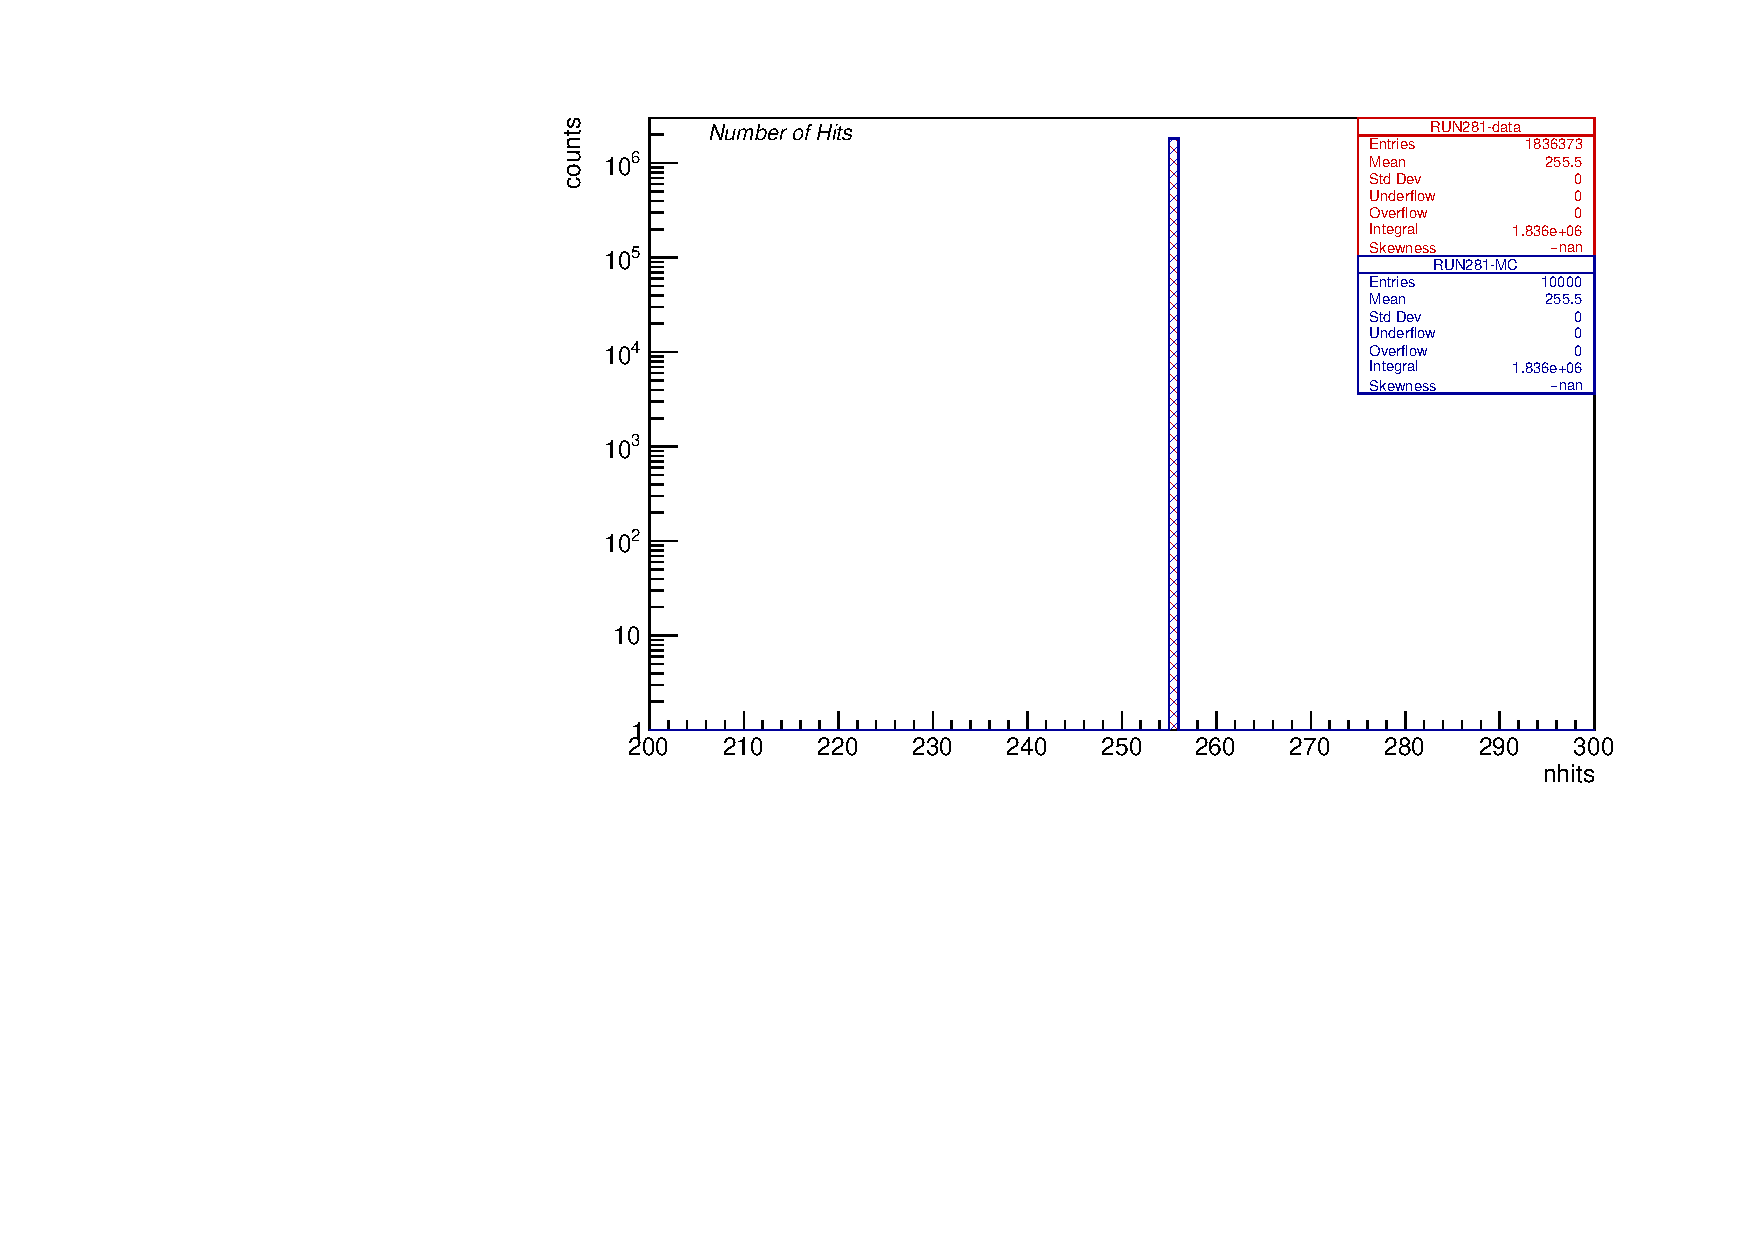
\includegraphics[width =0.8\textwidth]{figures/pdf/figure_00008_nhits_281}
\caption{
  \del{Total number of hits distribution.}
  \add{The distribution of the total number of hits read out per event}
}
\label{fig:3}
\end{figure}


%%% Local Variables:
%%% mode: latex
%%% TeX-master: t
%%% End:
